The current implementation, while functional, is far from optimal. There are bottlenecks which restrict performance and the system is unstable. It is not feasible to build a system as fast and as performant and stable as \ceph{} or \ac{hdfs} within the scope of a thesis. Experimenting around these limitations we can still answer the question we posed in the introduction. It being: can an architecture using ministries together with ranged based file locking offer an advantage over existing approaches.

To design experiments that work around the limitations we need to be clear on what the limitations are:

\begin{itemize}
	\item The \raft{} implementation sends only a single log entry at the time and log entries are sent each heartbeat period instead of whenever data becomes available. Effectively this imposes a rate limit on changing the systems metadata.
	\item Load balancing only replaces nodes that go down, it does not perform subtree partitioning at runtime (see:~\Cref{sec:subtree}).
	\item Sometimes nodes become unresponsive when making many requests that change metadata. They then miss heartbeats which triggers re-elections.
\end{itemize}

In \cref{sec:res_arg} we look at the \textit{ministry architecture} tracking how performance changes when we change the number of ministries. Then we look at \textit{ranged based file locking} in \cref{sec:res_range}, we compare write performance with and without locking. In each section I will detail how the experiments work around the limitations, ensuring their outcome would match an implementation without restrictions. Every benchmark was performed five times and all the results are presented. The nodes where monitored during each run and if an error occurred we repeated the entire run. When using multiple clients to create a larger load the nodes where given time to initialize and the test start was synchronized. All raw data is available at \href{https://github.com/dvdsk/Thesis}{github.com/dvdsk/Thesis}.

The benchmarks have been performed using the fifth generation distributed ASCI Supercomputer \cite{das5}. Each node has a dual eight-core Intel Xeon E5-2630 v3 cpus and 125G of ram. As networking delays are a key characteristic of the systems' performance we used Ethernet for the communication between nodes even though the hardware is equipped with InfiniBand. The Raft heartbeat duration was set to 75 milliseconds for all tests.

\subsection{Ministry Architecture} \label{sec:res_arg}
Here we test the impact of varying the number of ministries on performance. We expect to see an almost linear improvement with more ministries given optimal size and shape of the load.

As discussed live subtree partitioning is still unimplemented, we work around this by implementing static subtree partitioning. The load balancer starts by initializing a single ministry responsible for the root directory. Additional static ministries can be passed through command line parameters. For these test we let it initialize n-1 extra ministries at paths \textsl{/n}. Including the root ministry (it must always be present) there are now n ministries available for testing.

\subsubsection*{List directory}
The first load we try is list directory. We perform 60 thousand list requests spread across all root directories from 30 clients concurrently. Each client sends the requests one after another as fast as possible. To keep the overhead from sending back the directory content small each directory contains only 10 files. The client processes are spread between 3 physical nodes.

The 2000 requests each client sends can be in two different orders: \textit{batch} and \textit{stride}. In \textit{batch} a client performs all the requests for a single directory before sending those for the next. When using the \textit{stride} pattern a client sends a request to the first directory and then sends the next request to another directory. There were a few extreme outliers, these where further out then 4 standard deviations. They are not shown in the plots. % TODO: change test, make batch and stride orders random such that they dont all hit ministry one first... <08-08-22> 

In \Cref{fig:ls_vs_ministries} we see a violin plot comparing the two request orders for clusters with various number of ministries. On the Y-axis we see the time it took a single request to complete. A wider distribution means more requests where completed within the same time. Note the multimodal distribution, the increasing duration for the slowest requests as the number of ministries increases and the difference in the fastest times between batch and stride.

\Cref{fig:ls_cdf} shows \acp{cdf} of clients performing 60 thousand list directory requests in \textit{batch} mode for varying amount of ministries. On the Y-axis are the proportion of requests that complete within the time on the X-axis. Note using \textit{one} ministry is always the fastest followed initially by a configuration using \textit{five} ministries until 80\% of requests complete. Past 80\% the second place it taken by the configuration with \textit{two} ministries.

\begin{figure}[bp]
	\centering
	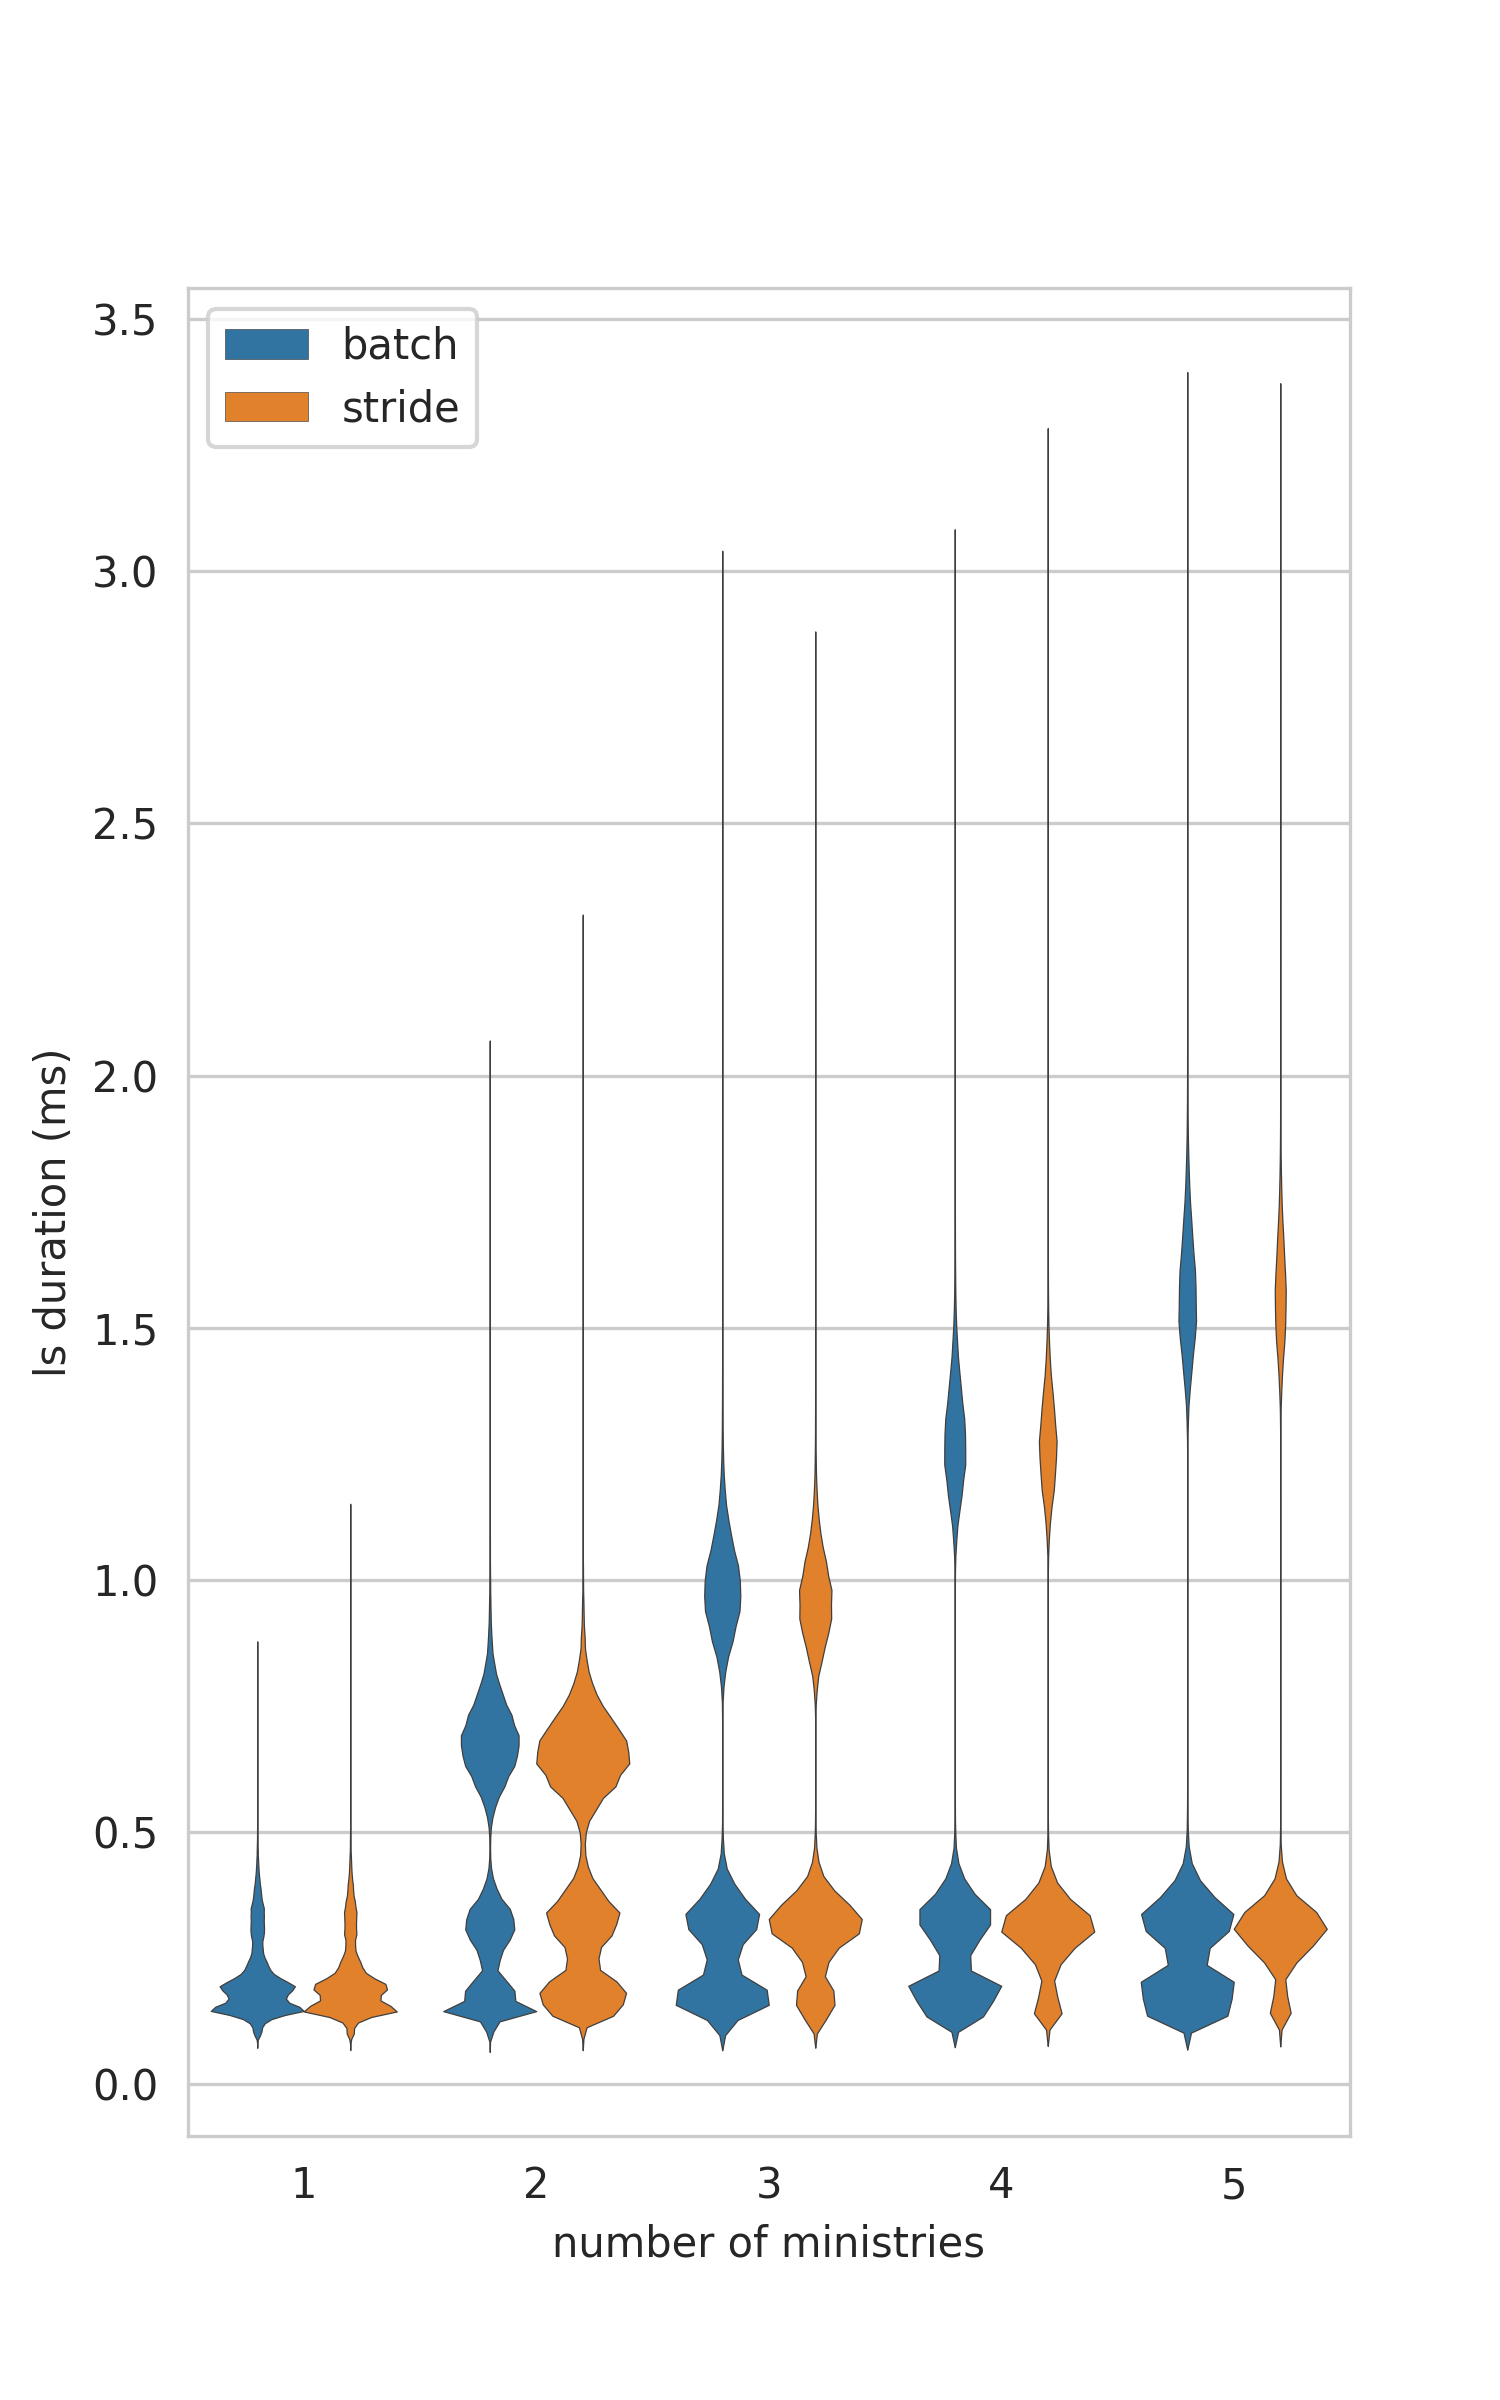
\includegraphics[height=\textheight]{../results/plots/ls_vs_numb_ministries.png}
	\caption{Distribution of list directory duration vs number of ministries for two different request orders. On the Y-axis the time it takes a single request to complete. The X-axis shows the number of ministries the file system is using. The orange distributions are results from runs where $30$ clients ordered their request such that the ministries where accessed one after the other, a stride pattern. The blue distributions show results from runs where $30$ clients used a batch pattern: they first perform all requests for one ministry and then for the next. Outliers further out then $4\sigma$ are not shown}
	\label{fig:ls_vs_ministries}
\end{figure}%

\begin{figure}[htb]
	\centering
	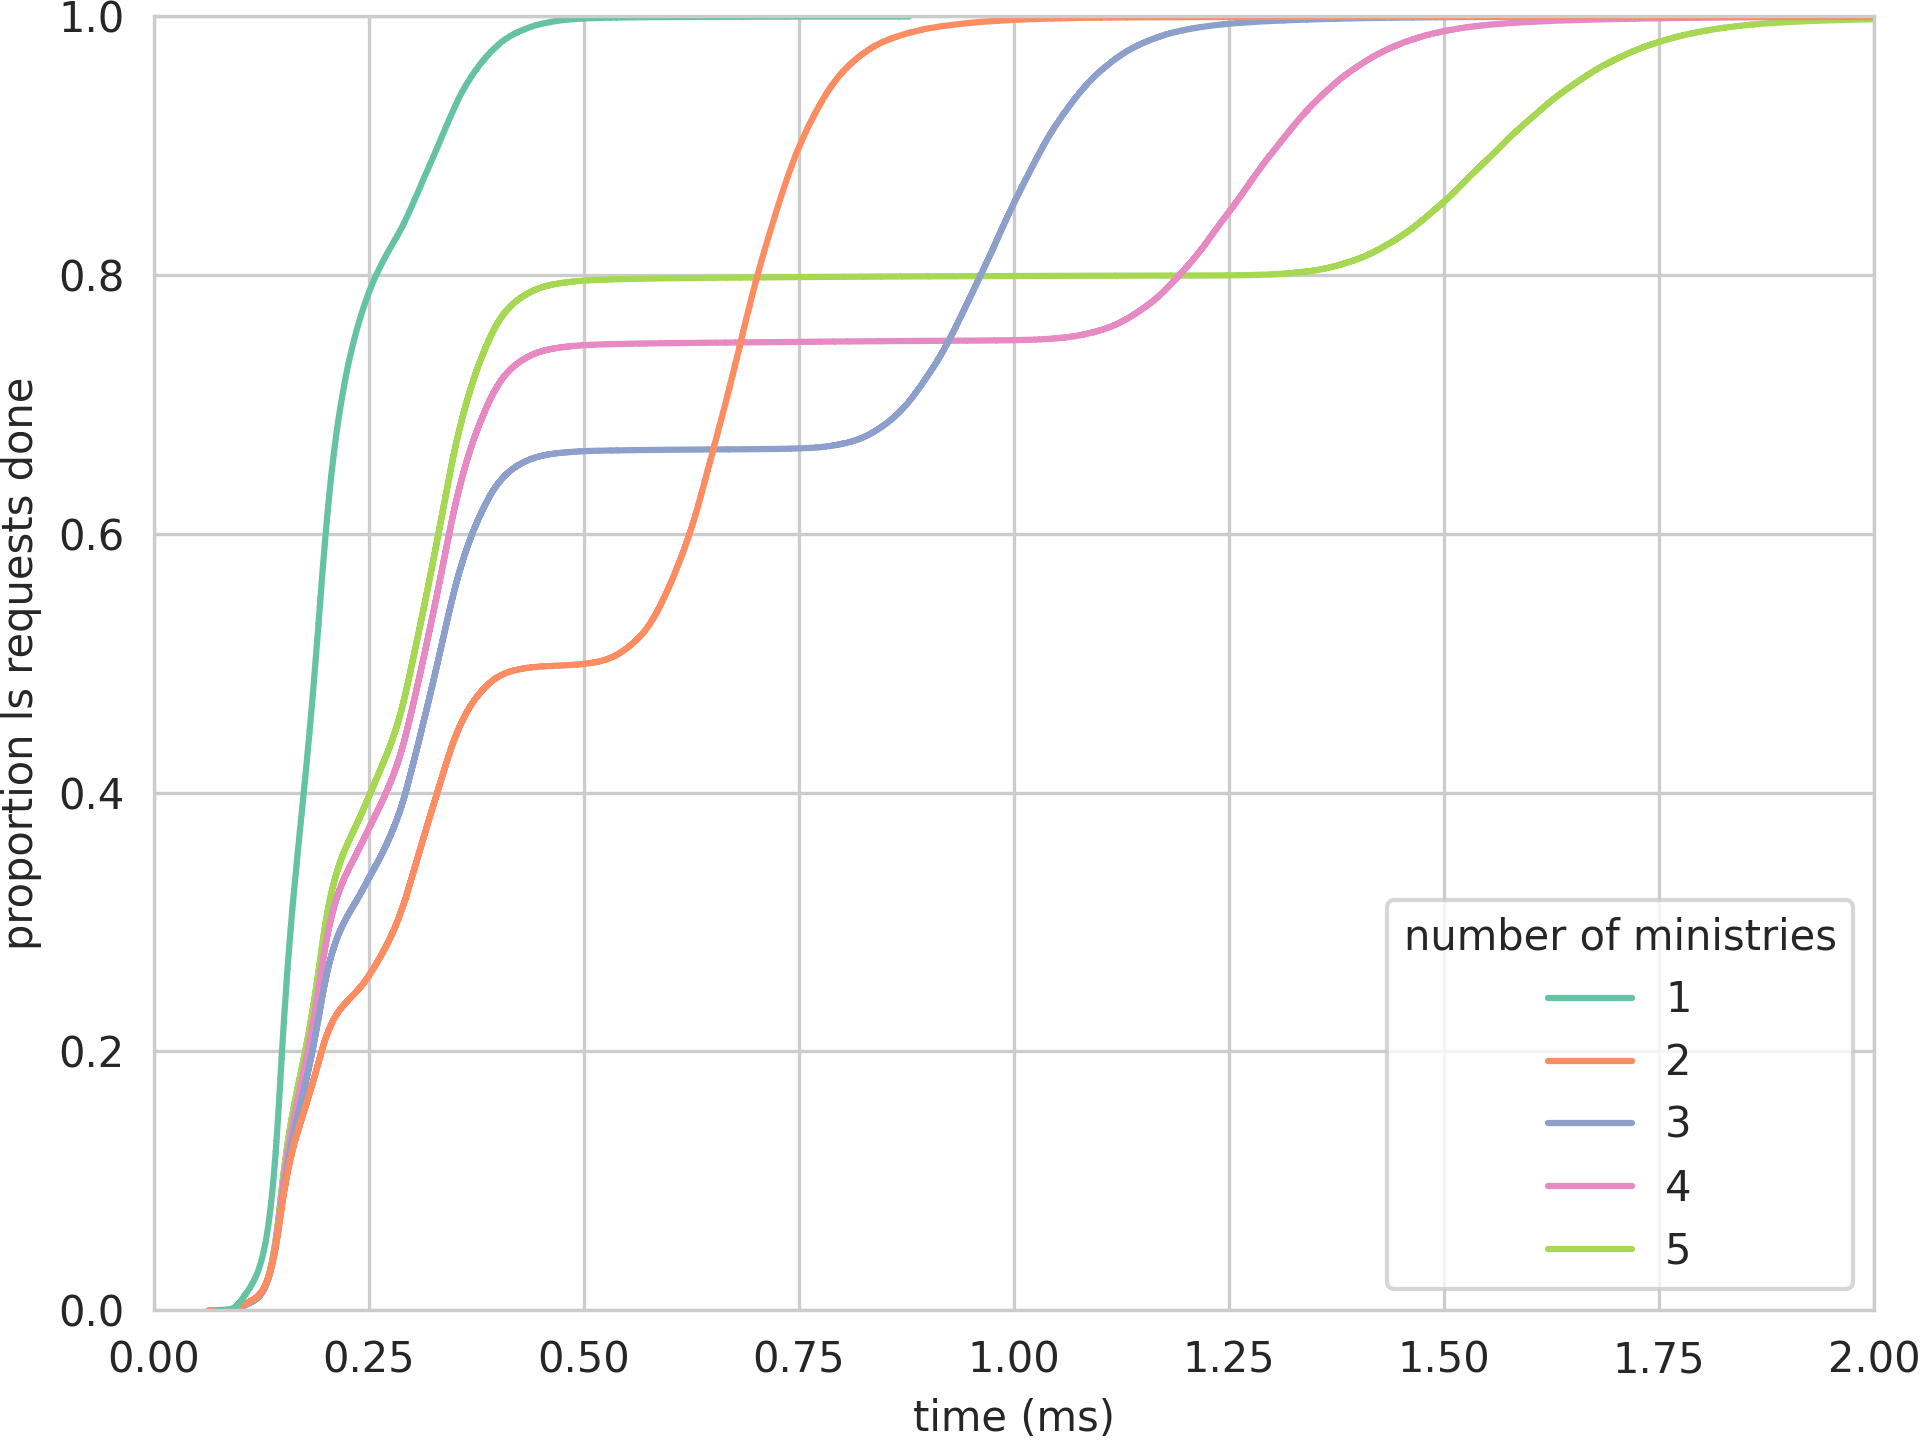
\includegraphics[height=\textheight]{../results/plots/ls_batch.png}
	\caption{\acp{cdf} of clients performing 60 thousand list directory requests for varying amount of ministries. On the Y-axis the proportion of requests completed, at $1.0$ all 60 thousand requests have been answered. The X-axis shows the time until the proportion was reached. The clients batch ordered their requests: they first perform all requests for one ministry and then for the next. The chart goes up to two milliseconds, a tiny fraction of requests take longer then that.}
	\label{fig:ls_cdf}
\end{figure}

\clearpage{}
\subsubsection{Create file*}
The second load we try is creating files. To create a file a minister appends a single message to the log making creating files rate limited. Without the rate limit load could increase until the communication with the clerks or the hardware of the nodes becomes the bottleneck.%
%\footnote{That is assuming there are no other bottlenecks. We investigate this by profiling the nodes, see:~\Cref{sec:profile}} % % TODO: re-enable if we have time/it is possible to present the profiling results <04-08-22> 

As adding more ministries could alleviate future bottlenecks it is interesting to see how file create performance scales with the number of ministries even given with the rate limits.

Because of this limit imposed by the implementation we send only 90 create requests. They are sent from 9 clients concurrently. These numbers where empirically determined to maximize the load while keeping the cluster stable enough to complete all the tests.

In \Cref{fig:touch} we see \acp{cdf} for the time it takes to create a file on configurations with a various number of ministries. On the Y-axis the proportion of write requests completed, and the X-axis shows the time in milliseconds. Note the first jump upwards is about 75 milliseconds and all the other jumps are around multiples of 75. The more ministries we use the faster most requests are done. Finally, note the proportion of requests completed jumps up in discrete steps.

\Cref{fig:touch_vs_time} offers another look at the same data. Here we see the time needed for each create as a function of when the request started. Darker tones are requests from tests with more ministries. On the Y-axis we see the time needed to complete the request in seconds while on the (logarithmic) X-axis we see the time a create request was sent. The vertical jumps in the \ac{cdf} (\Cref{fig:touch}) show up as horizontal bands here. For example the lowest horizontal band are requests that took 75 ms which matches the first vertical jump. Note that the gap just after the start of the test.

\begin{figure}[htbp]
	\centering
	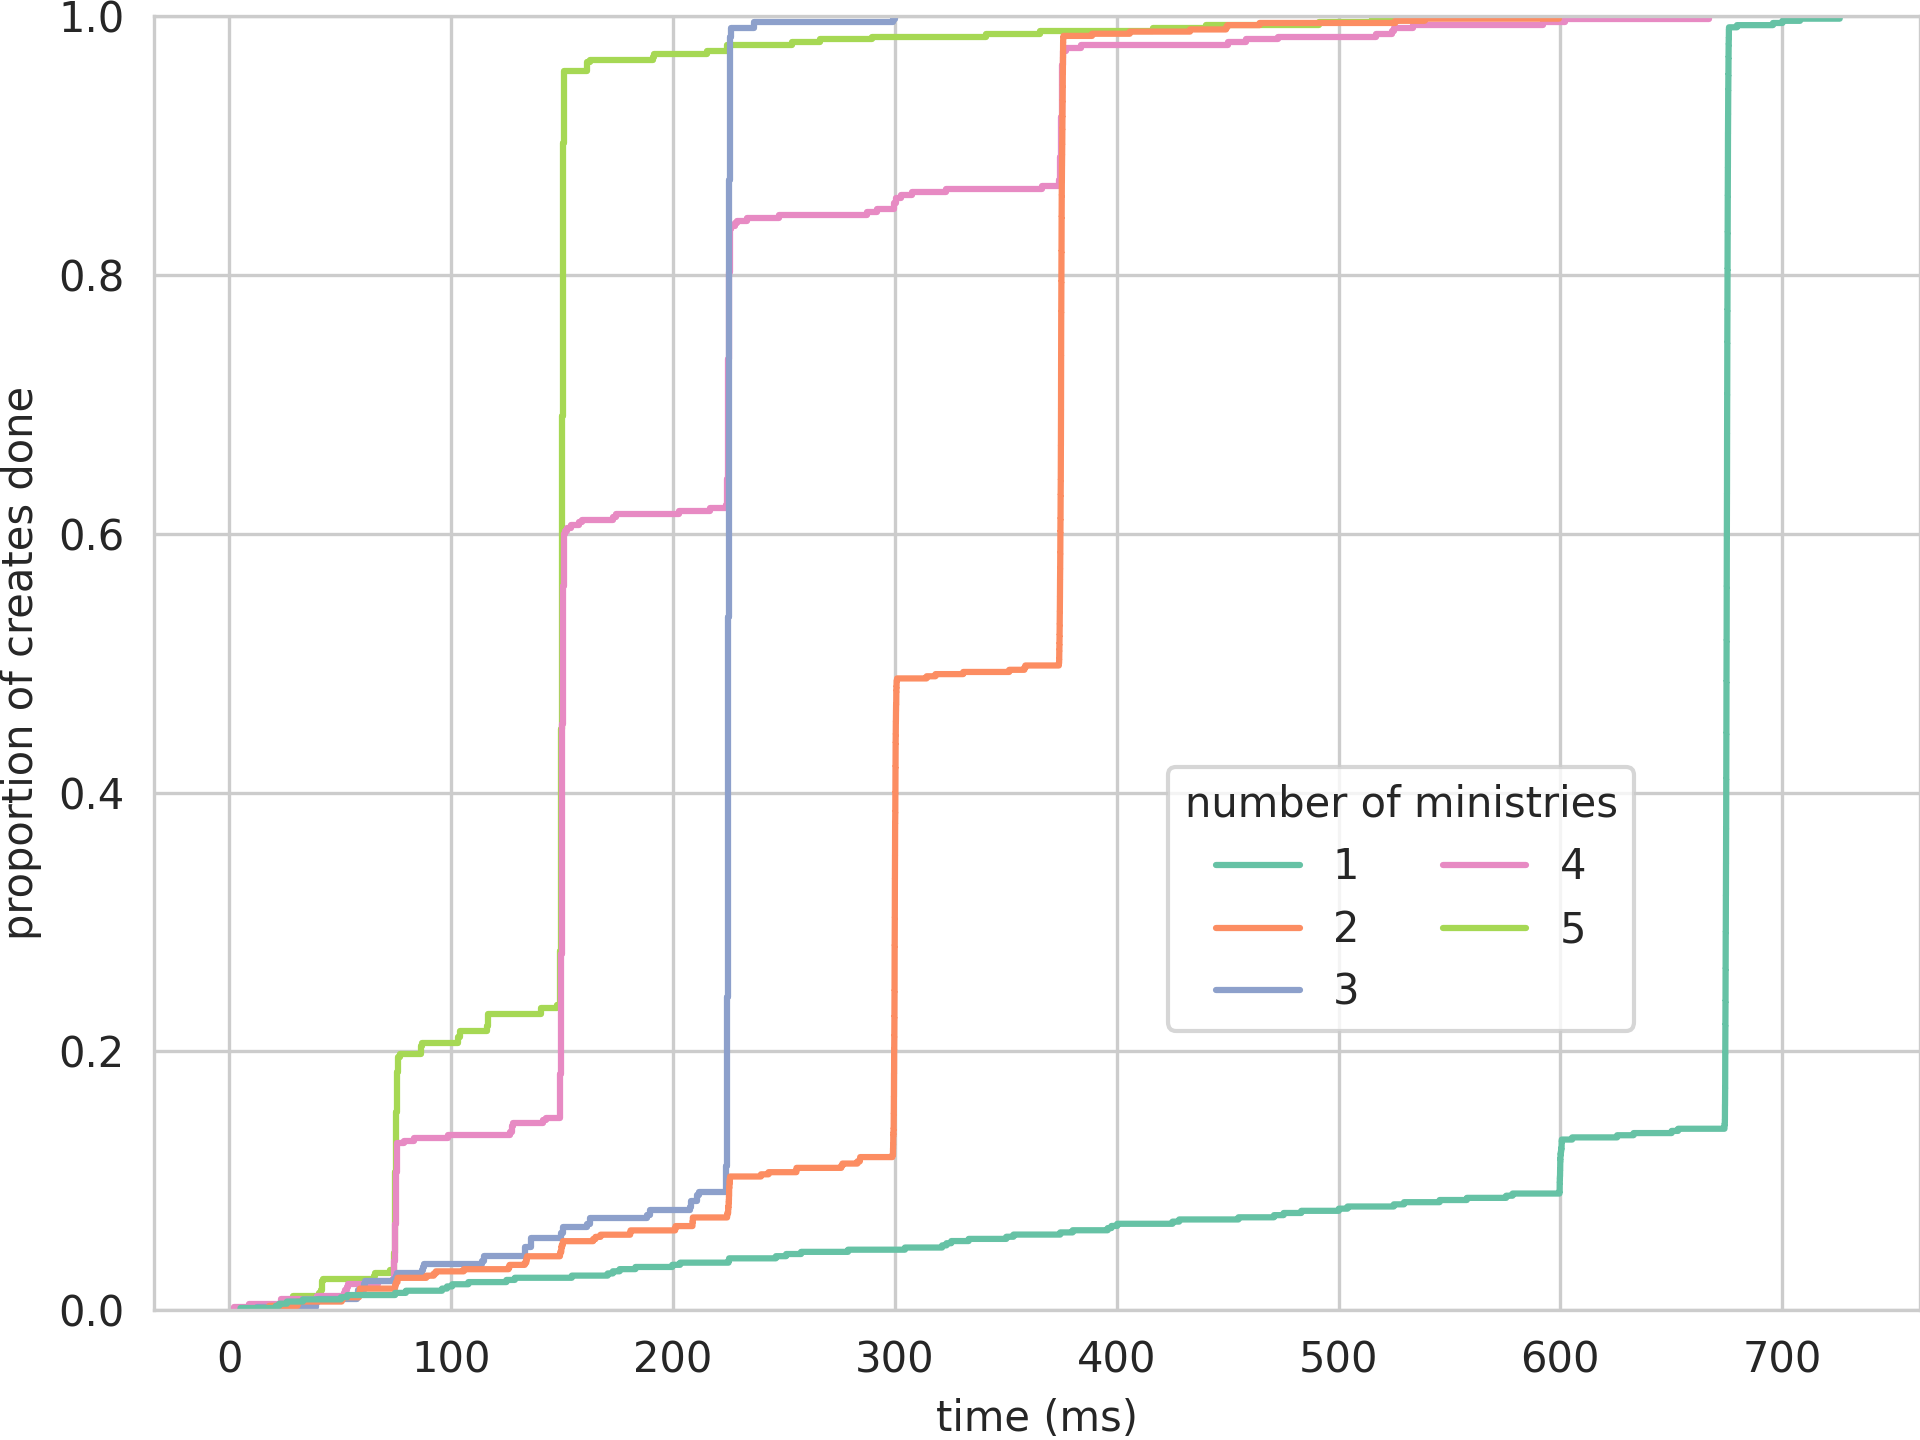
\includegraphics[height=\textheight]{../results/plots/touch.png}
	\caption{\acp{cdf} of clients creating 90 files on clusters with various amount of ministries. On the Y-axis the proportion of files created, at $1.0$ all 90 files have been created. On the X-axis the time in milliseconds until that proportion was reached.}
	\label{fig:touch}
\end{figure}

\begin{figure}[bp]
	\centering
	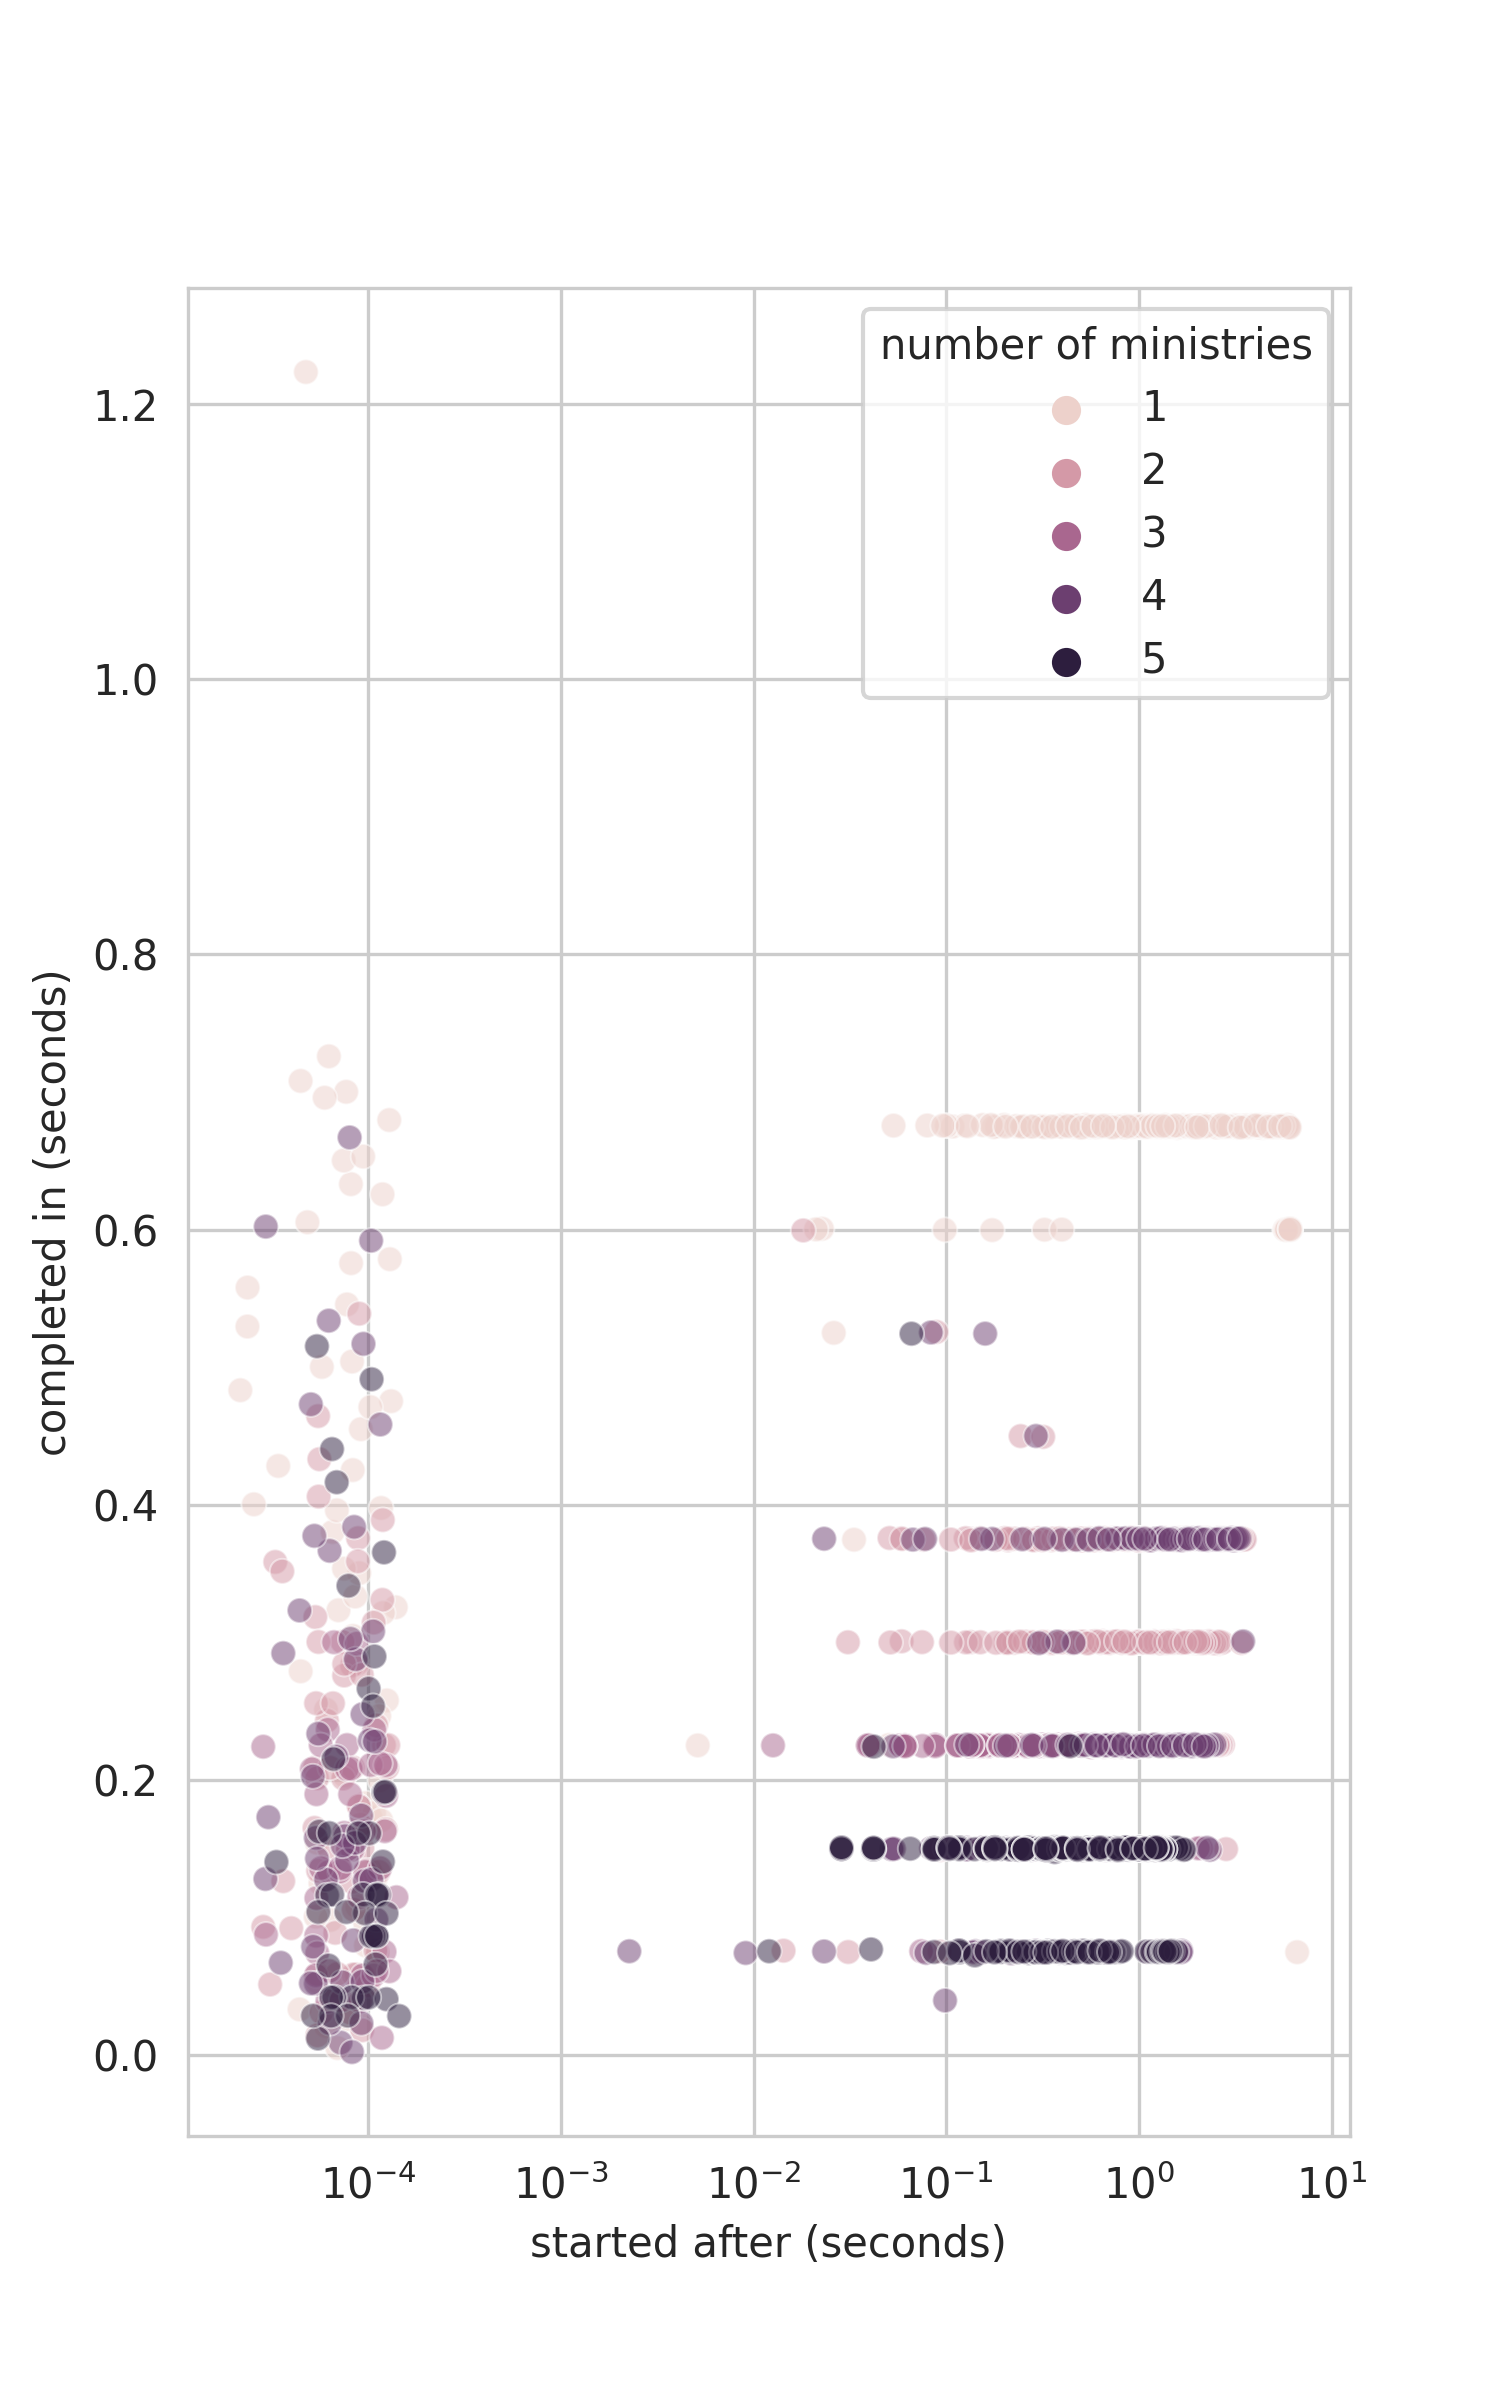
\includegraphics[height=\textheight]{../results/plots/touch_vs_time.png}
	\caption{A logarithmic plot of file create request time vs when the request was started. The same data as in \Cref{fig:touch}. On the Y-axis the time it took a request to complete in seconds while the X-axis shows the point at which the request was started. Darker points are from runs where the system had more ministiers.}
	\label{fig:touch_vs_time}
\end{figure}

\clearpage{}
\subsection{Range based file locking} \label{sec:res_range}
Now we evaluate the contribution of ranged writes compared to writing the entire file. A good use case of ranged file access is writing out one or more rows in a file. In other systems we request exclusive access to the entire file and writing out all the needed rows. Here we can request access to and writ out one row at the time. We expect this second method to be faster when contending with more clients for the same file and with larger files.

Here we compare these methods using two different experiments. In the first experiment we write a single row of a file with 10 rows from multiple clients simultaneously. Each client picks a row at random. In the second experiment we write all rows. Each client uses a random order when writing by row.

We run both experiments for various row size and number of concurrent writers. When varying the row size the number of concurrent writers was fixed at six. While changing the number of writers the row size was kept at 10 \ac{mby}.

Since \name{} has no data plane implementation writing is simulated by sleeping on the client side. We simulate writing at a speed of 200 \ac{mby} per second\footnote{This corresponds to a slow hard drive. That is the best case scenario for writing by row since it increases the ration of time writing versus connecting and locking.}.

In the table below we see the time spend on simulating IO and the average duration for writing one or 10 rows either by locking the whole file or locking by row:
%
\begin{tabular}{lcccccc} \toprule
	& \multicolumn{6}{c}{Row Size (\ac{mby})} \\ \cmidrule(r){2-7}
	                   & 0.1 & 1 & 10 & 20 & 40 & 80 \\ \midrule
	Writing a single row  \\ \cmidrule(r){1-1}
	IO simulation (ms) & 0.5          & 5          & 50          & 100         & 200         & 400 \\
	Lock by row & 411 & 370 & 366 & 444 & 636 & 971\\
	Lock entire file & 62 & 114 & 298 & 618 & 975 & 1644 \\
\smallskip \\
	Writing 10 rows (s)\\ \cmidrule(r){1-1}
	IO simulation & 0.005          & 0.05          & 0.50          & 1         & 2         & 4 \\
	Lock by row & 2.83         & 3.00       & 3.52        & 4.58        & 7.29        & 12.12 \\
	Lock entire file & 0.57         & 0.82       & 1.51        & 2.65        & 4.90        & 9.60 \\ \bottomrule
\end{tabular}
%
In the next two subsections we will look at these results in greater depth.
%
\subsubsection*{Writing a single row}
\Cref{fig:single_rowlen} shows the time it takes to write a single row for different row sizes. The Y-axis shows the duration a single write request takes in seconds. Each dot is a single measurement. We see that locking the entire file is slower than locking only the needed row. Note how increasing the row length shrinks the performance gap between these methods. Note furthermore that there are many outliers when locking by row.

\begin{figure}[htbp]
	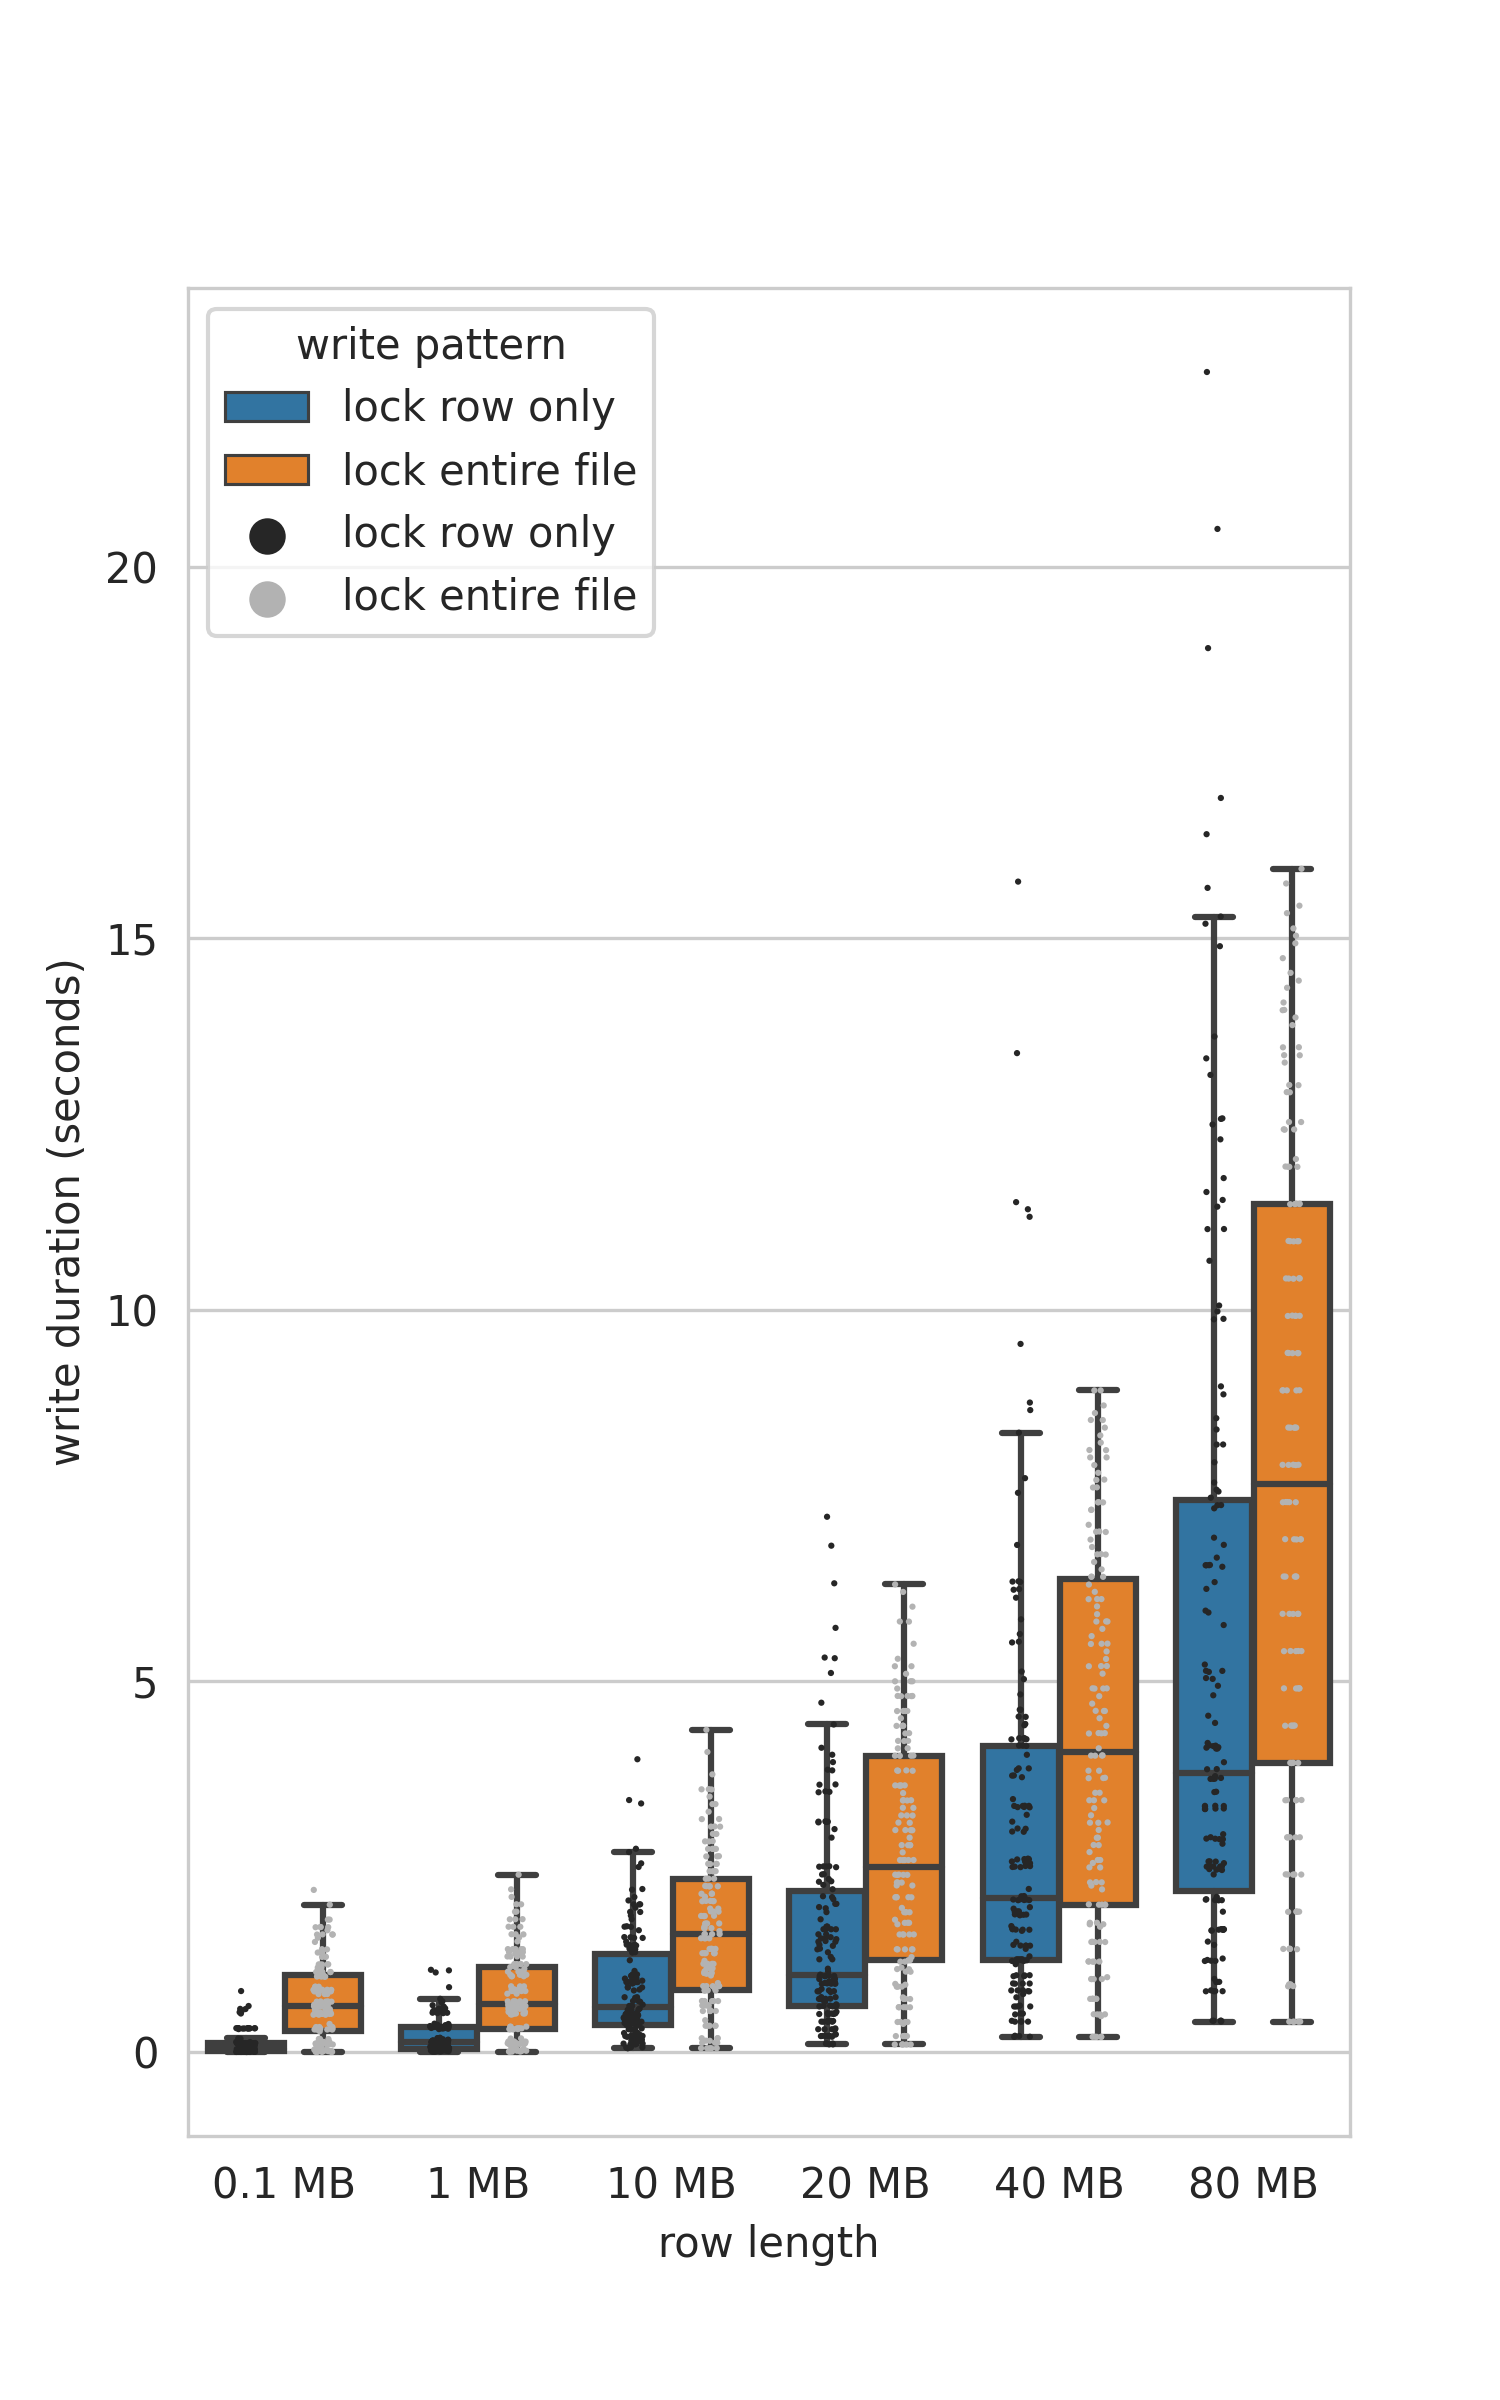
\includegraphics[width=3\textwidth]{../results/plots/single_vs_row_len.png}
	\caption{The time it takes to write a single row given different row sizes. Every dot is a single measurement. On the Y-axis the duration a single write request takes in seconds. On the X-axis the row size in MB. In blue the time needed when only locking the needed row while in orange we see the time needed when locking the entire file.}
	\label{fig:single_rowlen}
\end{figure}
%
In \Cref{fig:single_writers} we see that with more simultaneous writers locking only a single row becomes faster. The Y-axis shows the duration a single write request takes in milliseconds. Note how locking the entire file is faster up to and including 4 writers. This is strange as both methods lock the file once. The results where therefore ran thrice and triple checked.
%
\begin{figure}[htbp]
	\centering
	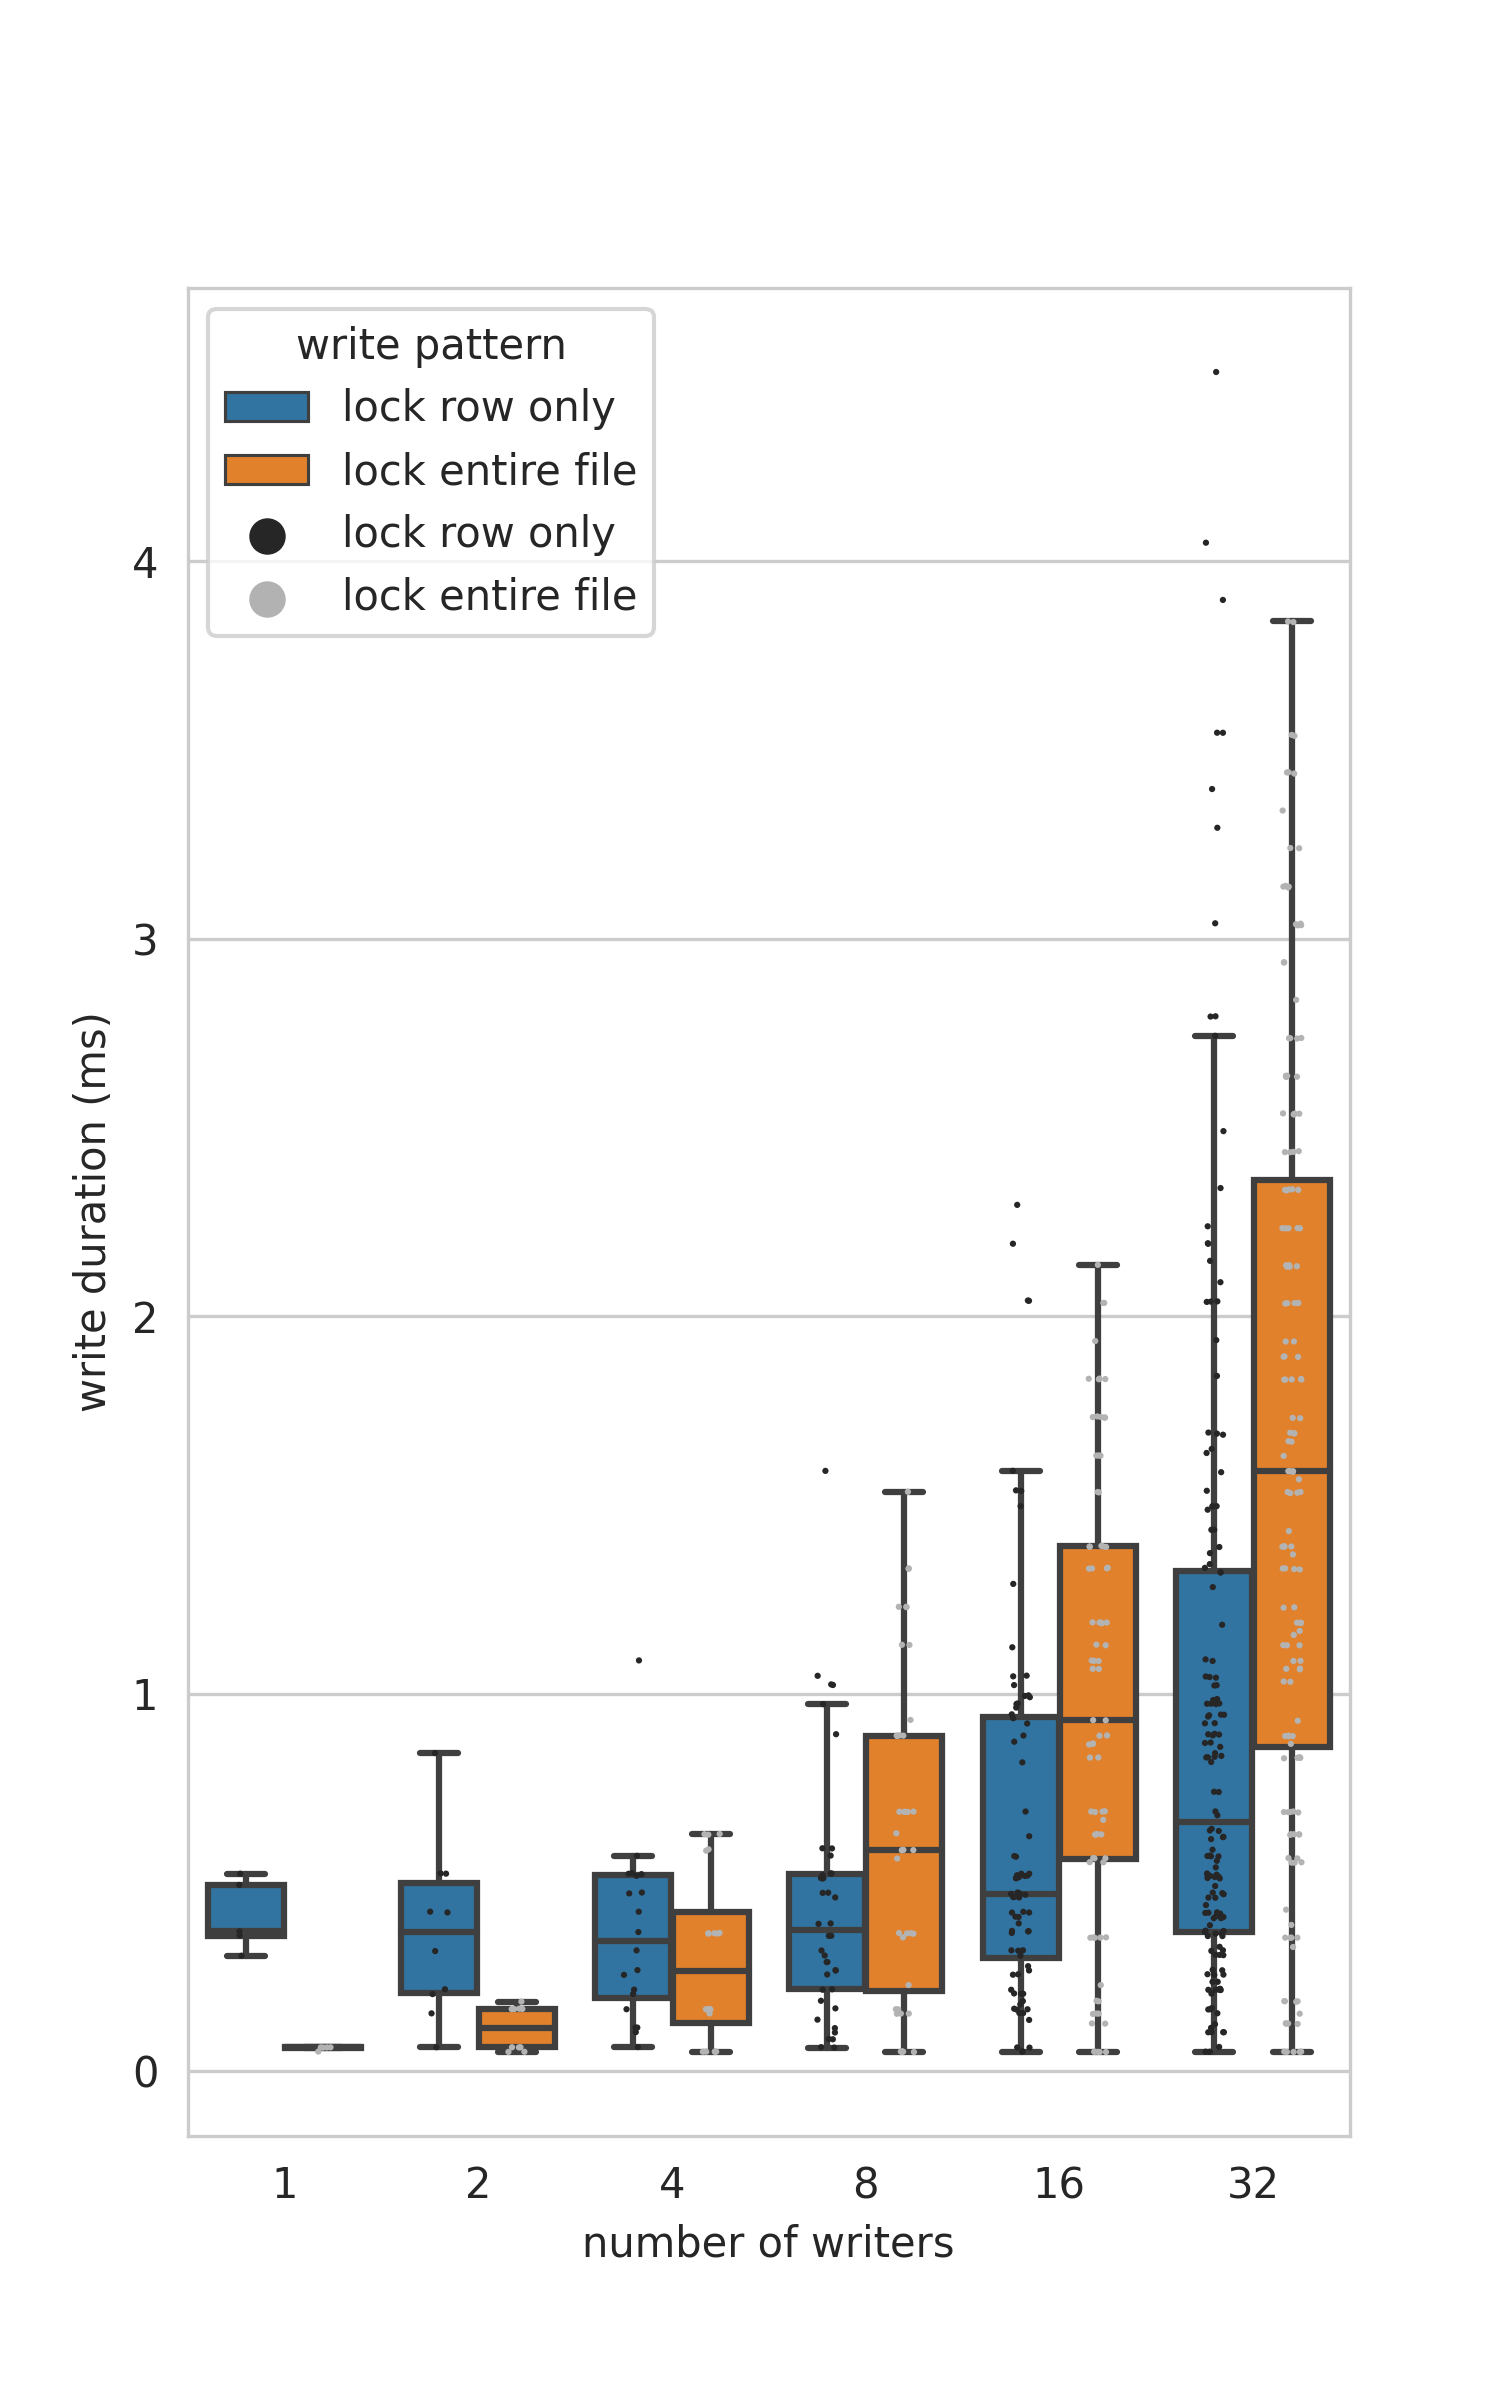
\includegraphics[height=\textheight]{../results/plots/single_vs_writers_both.png}
	\caption{The time it takes to write a single 10 \ac{mby} row given different numbers of writers from 1 to 32. On the Y-axis the duration in milliseconds. The X-axis shows the number of writers, doubling every time. In blue the time needed when only locking the needed row while in orange we see the time needed when locking the entire file.}
	\label{fig:single_writers}
\end{figure}

\clearpage
\subsubsection*{Writing the entire file}
In \Cref{fig:rowlen} we look at every individual duration measurement for writing all 10 rows given various row lengths. Again we compare locking by row versus locking the entire file. The logarithmic Y-axis shows the duration in seconds. The X-axis shows various sizes for the rows. As expected larger rows result in longer write durations. Furthermore, we see discrete levels in write duration when writing the entire file and not when writing by row.
%
\begin{figure}[htbp]
	\centering
	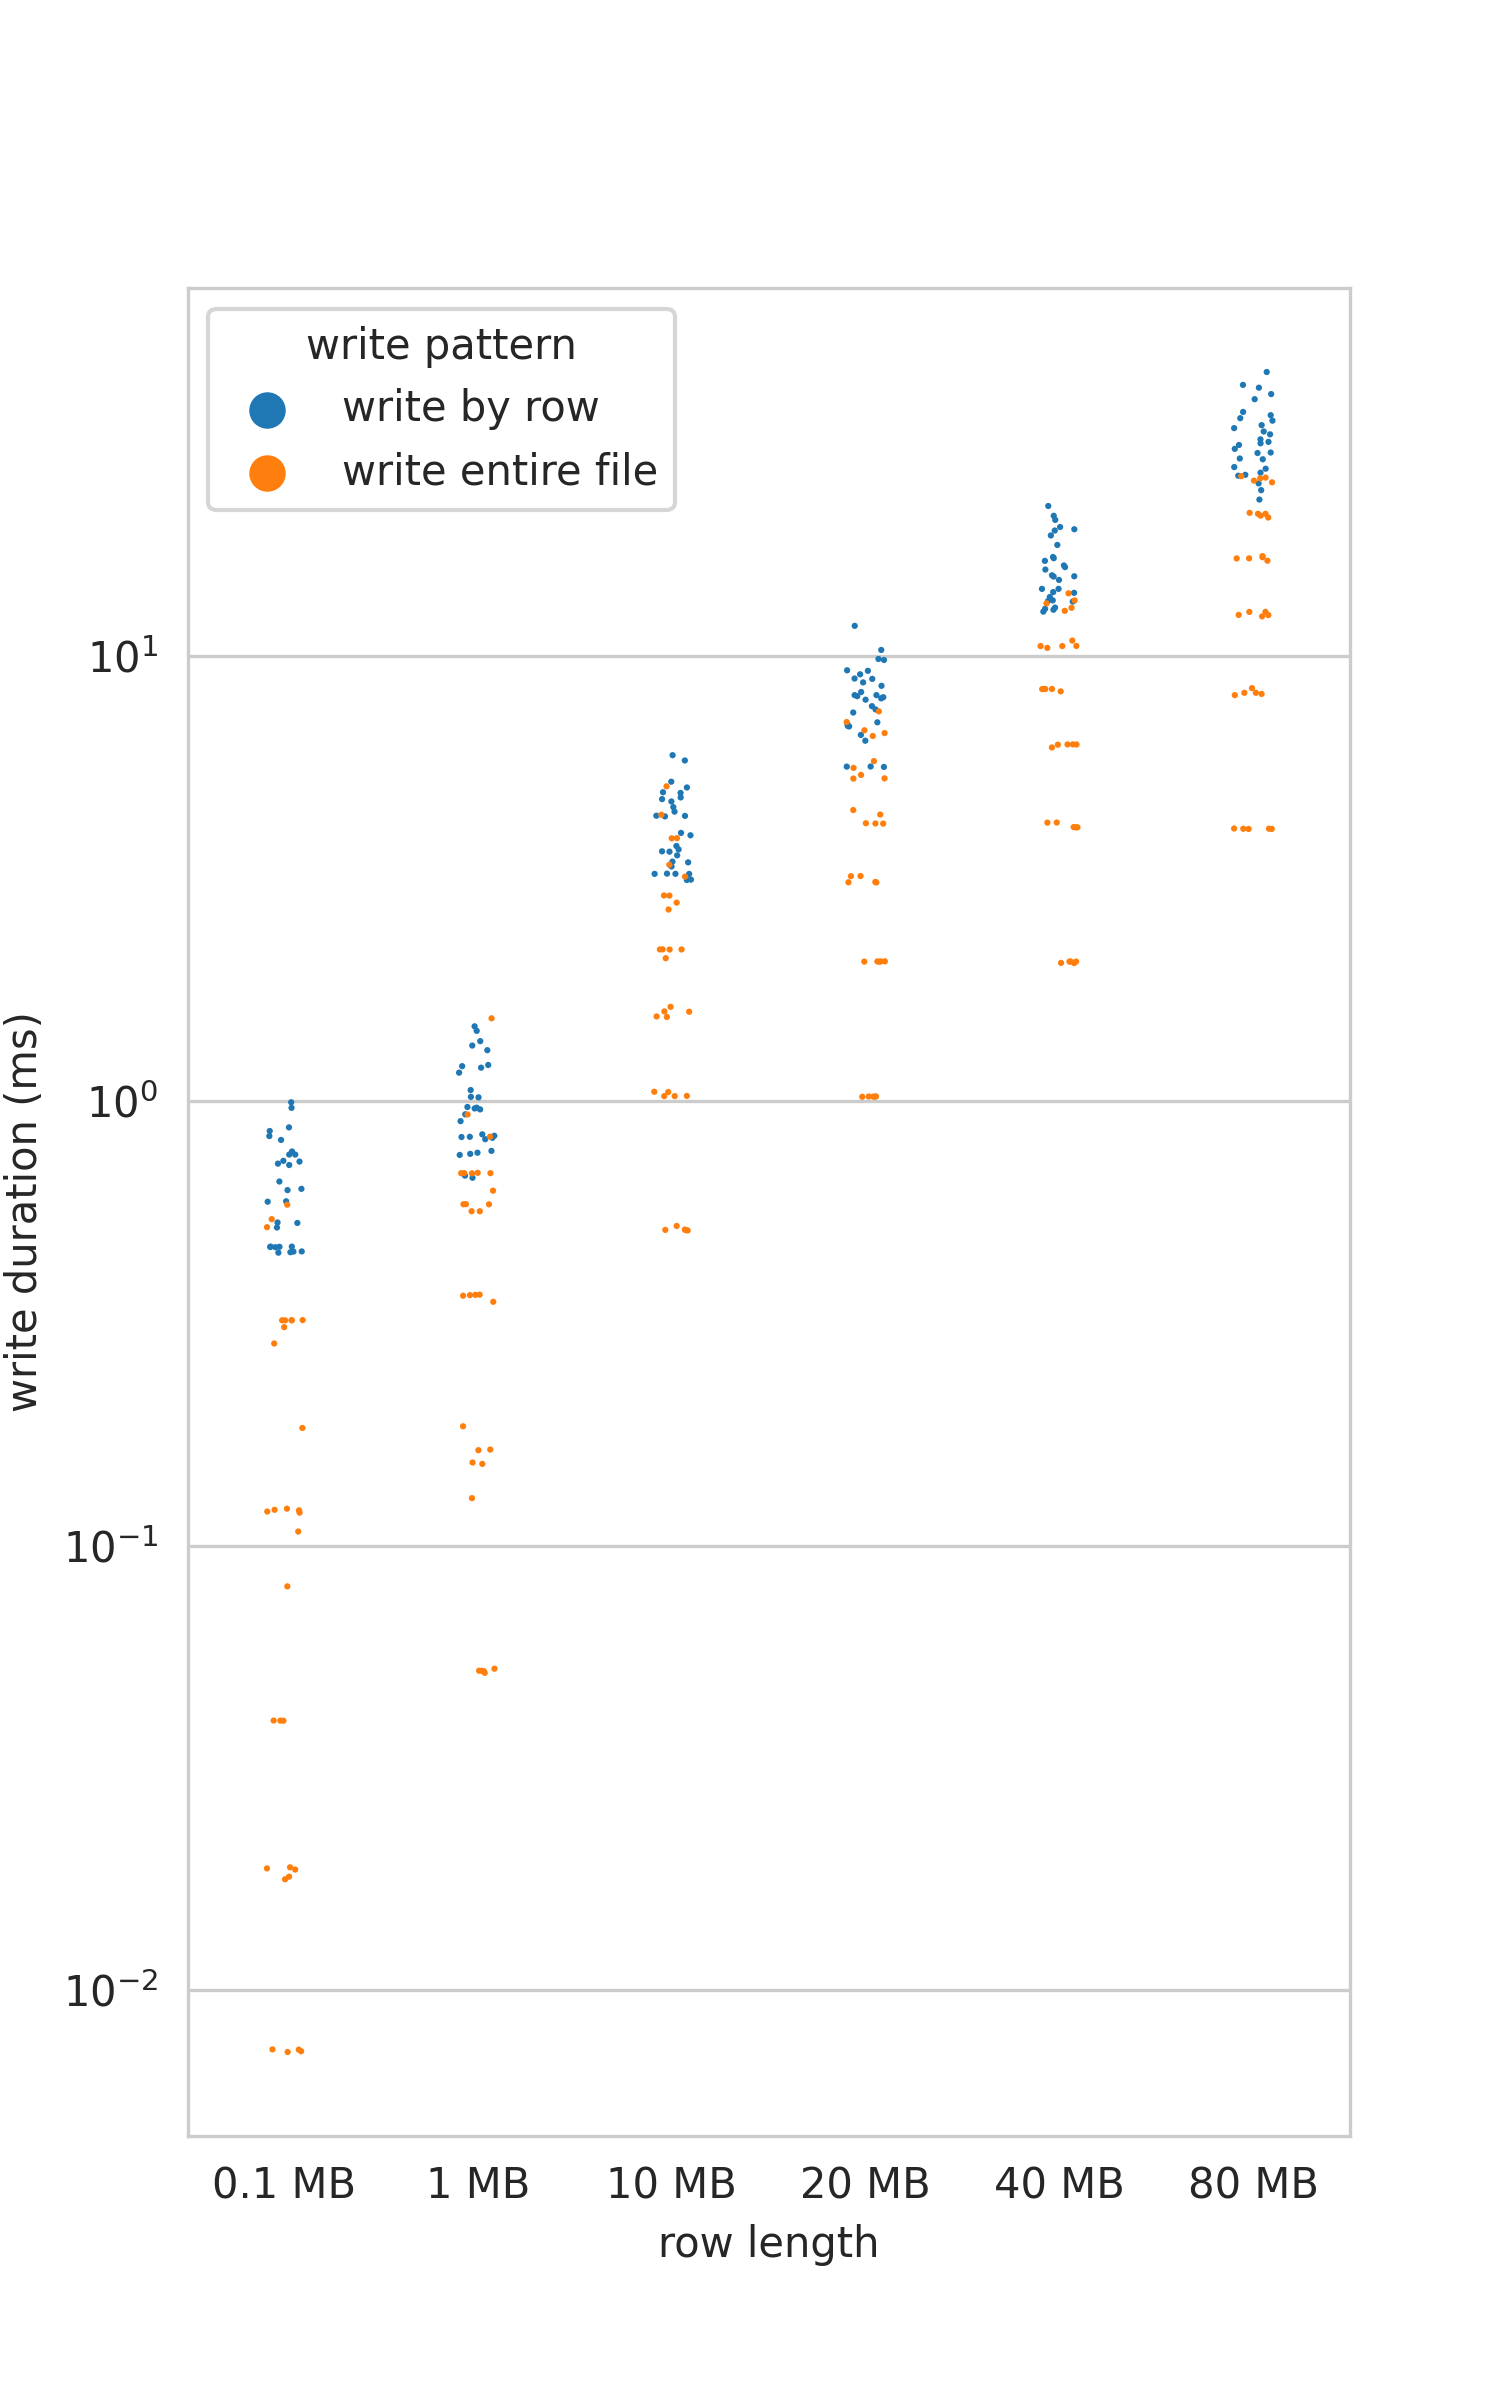
\includegraphics[height=\textheight]{../results/plots/range_vs_row_len.png}
	\caption{The time it takes to write 10 rows for varying row sizes. The blue dots are time measurements when only locking the needed row, locking in total ten times to write all rows. In orange the duration when locking the entire file and writing all rows at once.}
	\label{fig:rowlen}
\end{figure}%

\Cref{fig:writers} again shows the duration it takes to write all the rows this time for varying number of writers, comparing locking by row versus locking the entire file. The Y-axis shows the time it takes to write all 10 rows. Note how writing by row takes significantly longer with the gap closing when the number of writers increases. Also note the uniform distribution between the fastest and slowest time when locking the entire file (orange).
%
\begin{figure}[htbp]
	\centering
	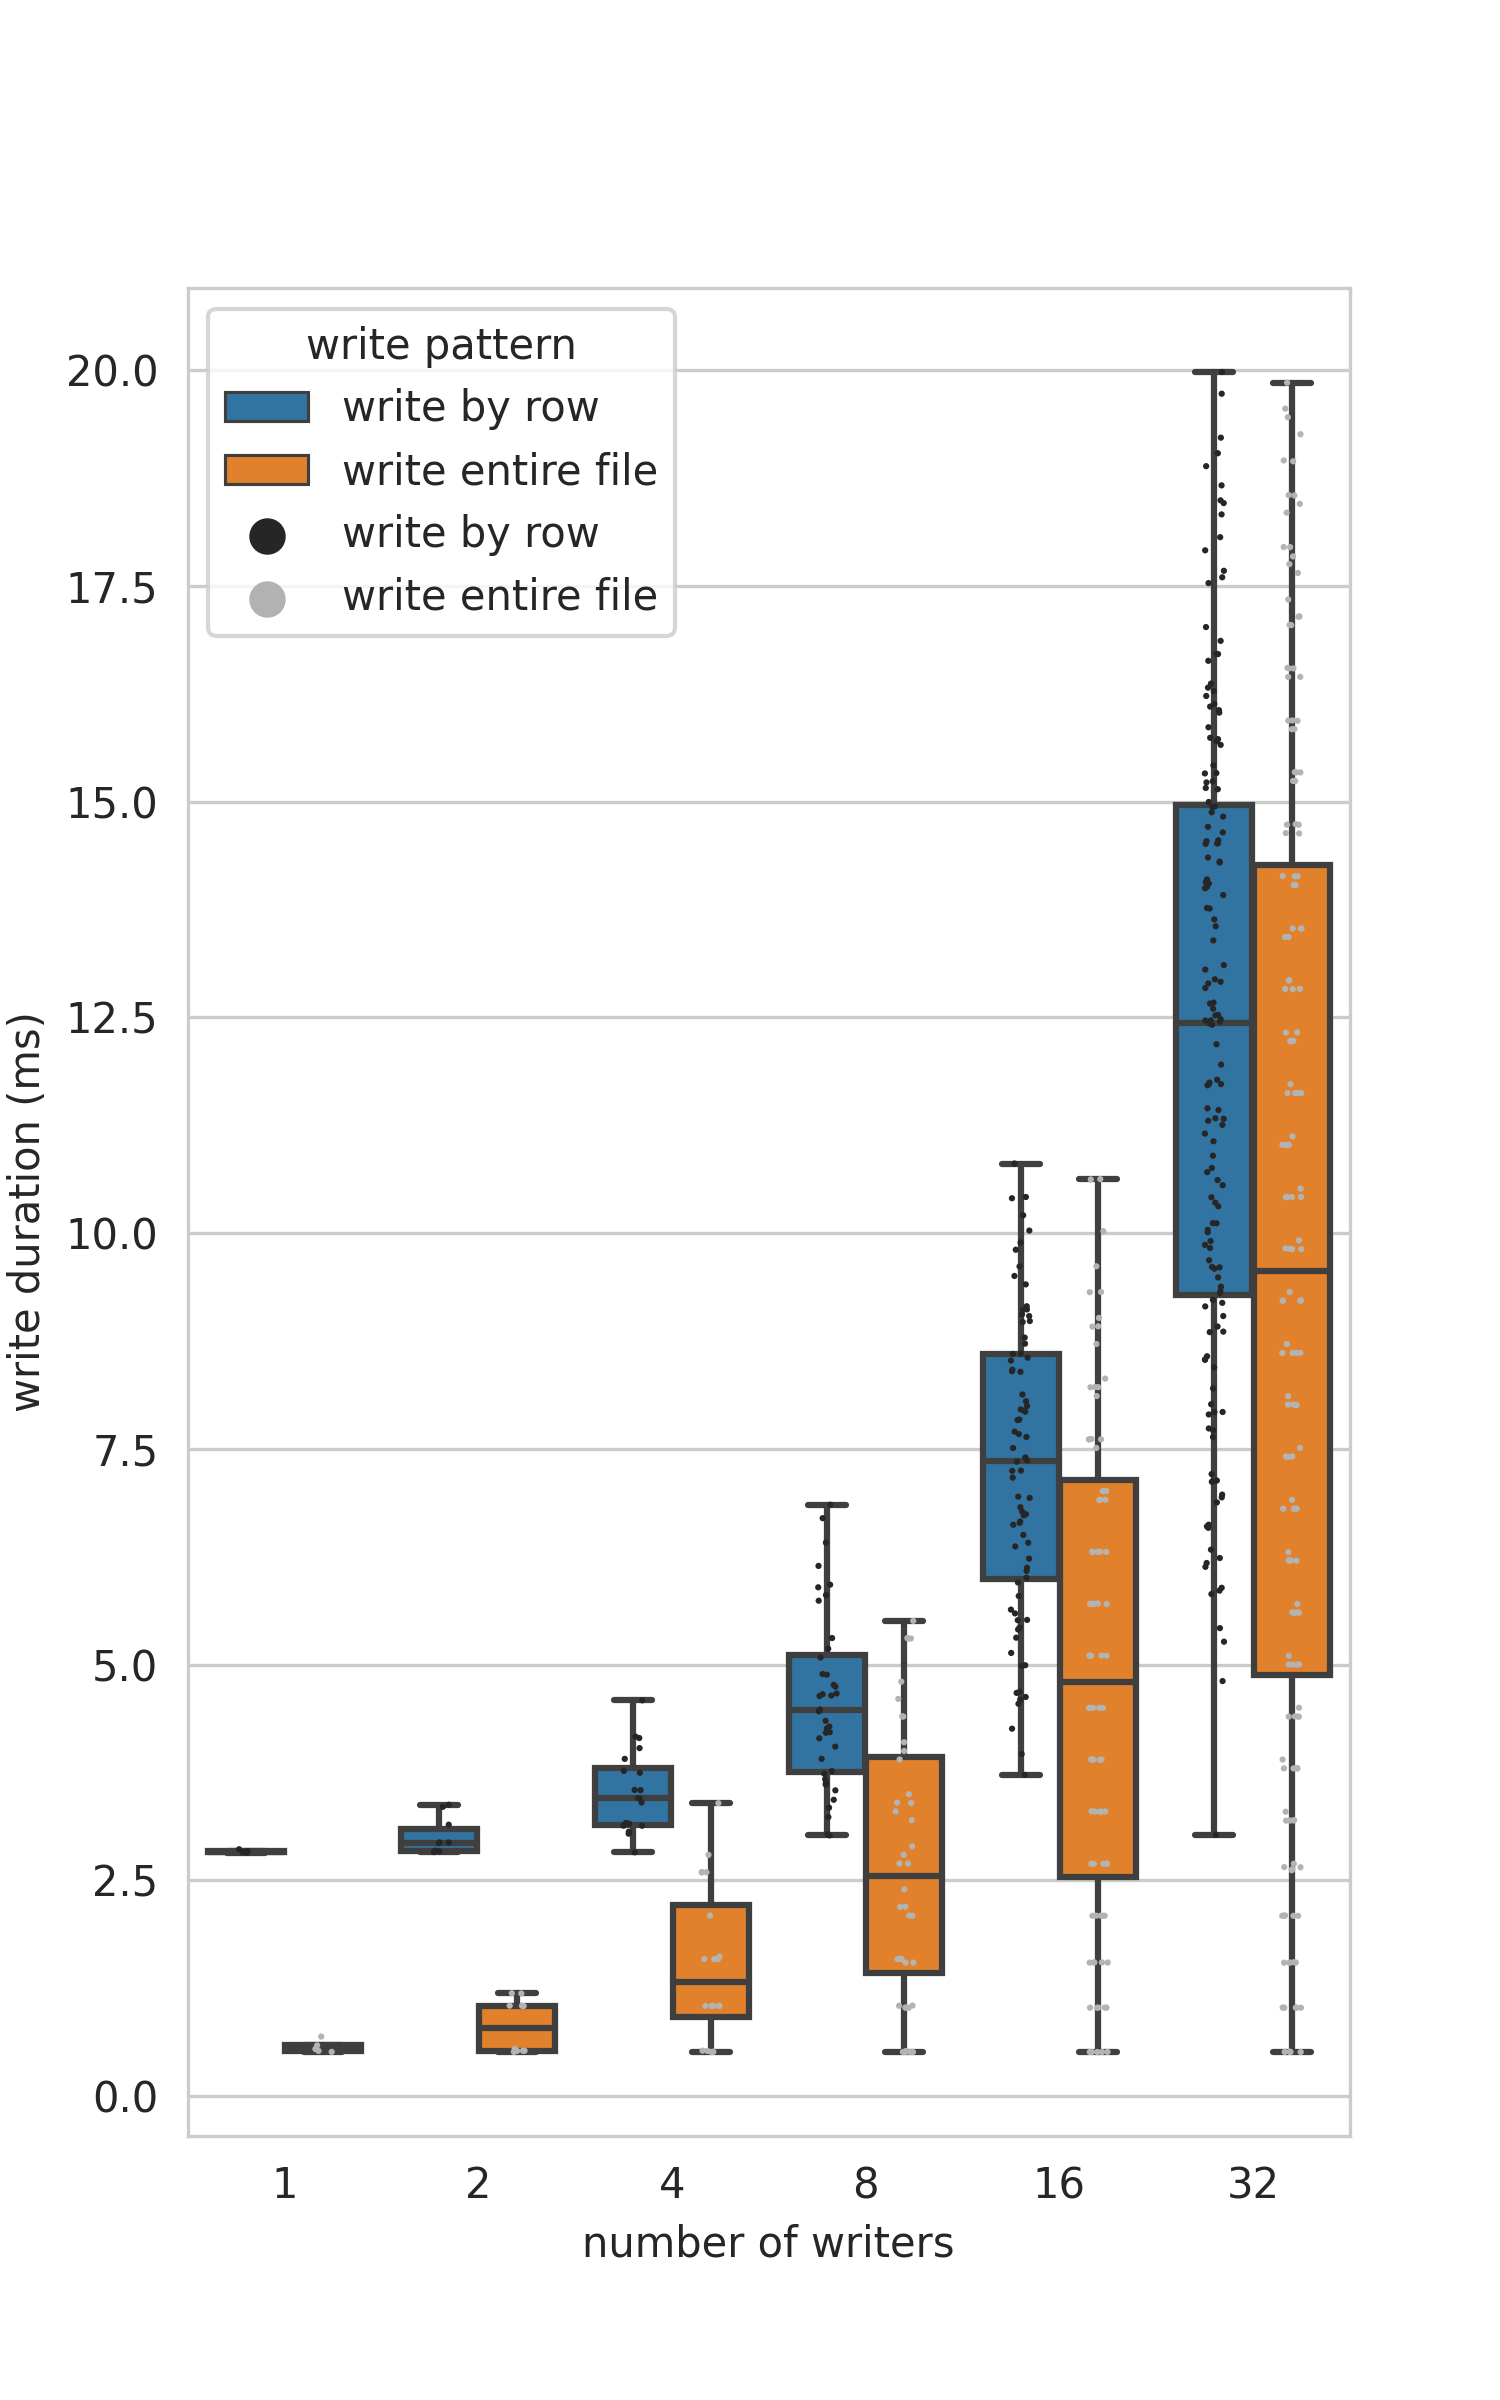
\includegraphics[height=\textheight]{../results/plots/range_vs_writers_both.png}
	\caption{The time it takes to write ten rows with between one and 32 concurrent writers. On the logarithmic Y-axis the duration in milliseconds. In blue the duration when only locking the needed row, locking in total ten times to write all rows. In orange the result when locking the entire file and writing all rows at once.}
	\label{fig:writers}
\end{figure}

\clearpage

%\subsection{Profiling} \label{sec:profile}
% for now we are not doing this (time limitations)
